%%%%%%%%%%%%%%%%%%%%%%%%%%%%%%%%%%%%%%%%%%%%%%%%%%%%%%%%%%%%%%%%%%%%%%%%%%%%%%%%%%%%%%%%%%%%%%%%%%%%%%
% Plantilla básica de Latex en Español.
%
% Autor: Andrés Herrera Poyatos (https://github.com/andreshp) 
%
% Es una plantilla básica para redactar documentos. Utiliza el paquete fancyhdr para darle un
% estilo moderno pero serio.
%
% La plantilla se encuentra adaptada al español.
%
%%%%%%%%%%%%%%%%%%%%%%%%%%%%%%%%%%%%%%%%%%%%%%%%%%%%%%%%%%%%%%%%%%%%%%%%%%%%%%%%%%%%%%%%%%%%%%%%%%%%%%

%-----------------------------------------------------------------------------------------------------
%	INCLUSIÓN DE PAQUETES BÁSICOS
%-----------------------------------------------------------------------------------------------------

\documentclass{article}


%-----------------------------------------------------------------------------------------------------
%	SELECCIÓN DEL LENGUAJE
%-----------------------------------------------------------------------------------------------------

% Paquetes para adaptar Látex al Español:
\usepackage[spanish,es-noquoting, es-tabla, es-lcroman]{babel} % Cambia 
\usepackage[utf8]{inputenc}                                    % Permite los acentos.
\selectlanguage{spanish}                                       % Selecciono como lenguaje el Español.

%-----------------------------------------------------------------------------------------------------
%	SELECCIÓN DE LA FUENTE
%-----------------------------------------------------------------------------------------------------

% Fuente utilizada.
\usepackage{courier}                    % Fuente Courier.
\usepackage{microtype}                  % Mejora la letra final de cara al lector.

%-----------------------------------------------------------------------------------------------------
%	ESTILO DE PÁGINA
%-----------------------------------------------------------------------------------------------------

% Paquetes para el diseño de página:
\usepackage{fancyhdr}               % Utilizado para hacer títulos propios.
\usepackage{lastpage}               % Referencia a la última página. Utilizado para el pie de página.
\usepackage{extramarks}             % Marcas extras. Utilizado en pie de página y cabecera.
\usepackage[parfill]{parskip}       % Crea una nueva línea entre párrafos.
\usepackage{geometry}               % Asigna la "geometría" de las páginas.

% Se elige el estilo fancy y márgenes de 3 centímetros.
\pagestyle{fancy}
\geometry{left=3cm,right=3cm,top=3cm,bottom=3cm,headheight=1cm,headsep=0.5cm} % Márgenes y cabecera.
% Se limpia la cabecera y el pie de página para poder rehacerlos luego.
\fancyhf{}

% Espacios en el documento:
\linespread{1.1}                        % Espacio entre líneas.
\setlength\parindent{0pt}               % Selecciona la indentación para cada inicio de párrafo.

% Cabecera del documento. Se ajusta la línea de la cabecera.
\renewcommand\headrule{
	\begin{minipage}{1\textwidth}
	    \hrule width \hsize 
	\end{minipage}
}

% Texto de la cabecera:
\lhead{\subject}                          % Parte izquierda.
\chead{}                                    % Centro.
\rhead{\doctitle \ - \docsubtitle}              % Parte derecha.

% Pie de página del documento. Se ajusta la línea del pie de página.
\renewcommand\footrule{                                 
\begin{minipage}{1\textwidth}
    \hrule width \hsize   
\end{minipage}\par
}

\lfoot{}                                                 % Parte izquierda.
\cfoot{}                                                 % Centro.
\rfoot{Página\ \thepage\ de\ \protect\pageref{LastPage}} % Parte derecha.


%----------------------------------------------------------------------------------------
%   MATEMÁTICAS
%----------------------------------------------------------------------------------------

% Paquetes para matemáticas:                     
\usepackage{amsmath, amsthm, amssymb, amsfonts, amscd} % Teoremas, fuentes y símbolos.
     
 % Nuevo estilo para definiciones
 \newtheoremstyle{definition-style} % Nombre del estilo
 {5pt}                % Espacio por encima
 {0pt}                % Espacio por debajo
 {}                   % Fuente del cuerpo
 {}                   % Identación: vacío= sin identación, \parindent = identación del parráfo
 {\bf}                % Fuente para la cabecera
 {.}                  % Puntuación tras la cabecera
 {.5em}               % Espacio tras la cabecera: { } = espacio usal entre palabras, \newline = nueva línea
 {}                   % Especificación de la cabecera (si se deja vaía implica 'normal')
 
 % Nuevo estilo para teoremas
 \newtheoremstyle{theorem-style} % Nombre del estilo
 {5pt}                % Espacio por encima
 {0pt}                % Espacio por debajo
 {\itshape}           % Fuente del cuerpo
 {}                   % Identación: vacío= sin identación, \parindent = identación del parráfo
 {\bf}                % Fuente para la cabecera
 {.}                  % Puntuación tras la cabecera
 {.5em}               % Espacio tras la cabecera: { } = espacio usal entre palabras, \newline = nueva línea
 {}                   % Especificación de la cabecera (si se deja vaía implica 'normal')
 
 % Nuevo estilo para ejemplos y ejercicios
 \newtheoremstyle{example-style} % Nombre del estilo
 {5pt}                % Espacio por encima
 {0pt}                % Espacio por debajo
 {}                   % Fuente del cuerpo
 {}                   % Identación: vacío= sin identación, \parindent = identación del parráfo
 {\scshape}                % Fuente para la cabecera
 {:}                  % Puntuación tras la cabecera
 {.5em}               % Espacio tras la cabecera: { } = espacio usal entre palabras, \newline = nueva línea
 {}                   % Especificación de la cabecera (si se deja vaía implica 'normal')
 
 % Teoremas:
 \theoremstyle{theorem-style}  % Otras posibilidades: plain (por defecto), definition, remark
 \newtheorem{theorem}{Teorema}[section]  % [section] indica que el contador se reinicia cada sección
 \newtheorem{corollary}[theorem]{Corolario} % [theorem] indica que comparte el contador con theorem
 \newtheorem{lemma}[theorem]{Lema}
 \newtheorem{proposition}[theorem]{Proposición}
 
 % Definiciones, notas, conjeturas
 \theoremstyle{definition}
 \newtheorem{definition}{Definición}[section]
 \newtheorem{conjecture}{Conjetura}[section]
 \newtheorem*{note}{Nota} % * indica que no tiene contador
 
 % Ejemplos, ejercicios
 \theoremstyle{example-style}
 \newtheorem{example}{Ejemplo}[section]
 \newtheorem{exercise}{Ejercicio}[section]

%-----------------------------------------------------------------------------------------------------
%	BIBLIOGRAFÍA
%-----------------------------------------------------------------------------------------------------

\usepackage[backend=bibtex, style=numeric]{biblatex}
\usepackage{csquotes}

\addbibresource{references.bib}

%-----------------------------------------------------------------------------------------------------
%	PORTADA
%-----------------------------------------------------------------------------------------------------

% Elija uno de los siguientes formatos.
% No olvide incluir los archivos .sty asociados en el directorio del documento.
\usepackage{title1}
%\usepackage{title2}
%\usepackage{title3}

%-----------------------------------------------------------------------------------------------------
%	TÍTULO, AUTOR Y OTROS DATOS DEL DOCUMENTO
%-----------------------------------------------------------------------------------------------------

% Título del documento.
\newcommand{\doctitle}{Ecuaciones diferenciales ordinarias}
% Subtítulo.
\newcommand{\docsubtitle}{Método del trapecio}
% Fecha.
\newcommand{\docdate}{1 \ de \ Enero \ de \ 2015}
% Asignatura.
\newcommand{\subject}{Métodos Numéricos II}
% Autor.
\newcommand{\docauthor}{Andrés Herrera Poyatos \\ Javier Poyatos Amador \\ Rodrigo Raya Castellano}
\newcommand{\docaddress}{Universidad de Granada}
\newcommand{\docemail}{}

%-----------------------------------------------------------------------------------------------------
%	RESUMEN
%-------------------------------					----------------------------------------------------------------------

% Resumen del documento. Va en la portada.
% Puedes también dejarlo vacío, en cuyo caso no aparece en la portada.
%\newcommand{\docabstract}{}
\newcommand{\docabstract}{En este texto puedes incluir un resumen del documento. Este informa al lector sobre el contenido del texto, indicando el objetivo del mismo y qué se puede aprender de él.}

\begin{document}

\maketitle

%-----------------------------------------------------------------------------------------------------
%	ÍNDICE
%-----------------------------------------------------------------------------------------------------

% Profundidad del Índice:
%\setcounter{tocdepth}{1}

\newpage
\tableofcontents
\newpage

%-----------------------------------------------------------------------------------------------------
%	SECCIÓN 1: MOTIVACIÓN
%-----------------------------------------------------------------------------------------------------

\section{Motivación: resolución de ecuaciones diferenciales ordinarias}

%-----------------------------------------------------------------------------------------------------
%	SECCIÓN 2: MÉTODO DEL TRAPECIO
%-----------------------------------------------------------------------------------------------------

\section{Descripción del método del trapecio}

	Considérese el problema de valores iniciales dado por la ecuación diferencial $y'(t) = f(t,y(t))$ sobre $[a,b]$ y la condición $y(a) = y_0$. Supóngase que se ha averiguado que el problema admite solución única. Dado $n \in \mathbb{N}$ y sea $h = \frac{b-a}{2}$, se pretende obtener un método numérico para aproximar la imagen de $y$ en los puntos $t_i = a + ih$ con $i = 0 \ldots n$. Denotaremos $w_i$ a la aproximación obtenida para el punto $t_i$, comenzando con $w_0 = y_0$. El objetivo es encontrar una fórmula que permita aproximar $w_k$ a partir de $w_{k-1}$ e iterar este proceso para obtener las $n$ aproximaciones.
	
	Utilizando la Proposición X, la solución de este PVI es la única solución de la siguiente ecuación
	
	\begin{equation}
		y(t)  = y_0 + \int_{t_0}^{t} f(s,y(s))) \ ds
	\end{equation}
	
	En este contexto se pueden aplicar los métodos de integración numérica para aproximar la integral que aparece en la segunda igualdad. Para ello supóngase que $f$ es diferenciable. En tal caso una obvia inducción concluye que $y$ es de clase infinito. Por tanto, se puede utilizar la fórmula del trapecio para integración numérica, obteniendo la siguiente igualdad
	
	\begin{equation}
		y(t_{1}) = y_0 + \frac{h}{2} \left[f(t_0,y_0) + f(t_1, y(t_1))\right] - \frac{h^3}{12}y^{3)}(\xi)
	\end{equation}


	donde $\xi \in [t_0, t_1]$. Ignorando el último sumando se obtiene la siguiente aproximación dada en (\ref{eq:app}), que tiene error $- \frac{h^3}{12}y^{3)}(\xi)$.

	\begin{equation} \label{eq:app}
		y(t_1) \approx w_1 = w_0 + \frac{h}{2} \left[f(t_0,w_0) + f(t_1, y(t_1))\right]
	\end{equation}

	El problema reside en que para aproximar el valor de $y$ en $t_1$ se debe conocer previamente dicho valor. En este contexto se plantean dos soluciones diferentes obteniendo dos métodos, denominados método del trapecio explícito e implícito respectivamente.
	
	\subsection{Método del trapecio explícito}
		
		Recuérdese en este punto el método de Euler para ecuaciones diferenciales ordinarias. Este método consiste en aproximar $y(t_{k+1})$ a partir de $w_k$ de la siguiente forma
		
		\begin{equation} \label{eq:euler}
			y(t_{k+1}) \approx w_{k+1} = w_k + h f(t_k,w_k))
		\end{equation}

		Esto es, se predice $y(t_{1})$ como el valor que toma en $t_1$ la recta tangente a $y$ en $t_0$. Repitiendo el proceso se obtiene la fórmula \ref{eq:euler}. El error de este método es....

		El método del trapecio explícito se obtiene al combinar el método de Euler con (\ref{eq:app}) para obtener la siguiente aproximación

		\begin{equation} \label{eq:app-exp}
			y(t_{k+1}) \approx w_{k+1} = w_k + \frac{h}{2} \left[f(t_k,w_k) + f(t_{k+1}, w_k + h f(t_k,w_k))\right]
		\end{equation}

		Sauer
			
		\begin{figure}[h]
			\centering
			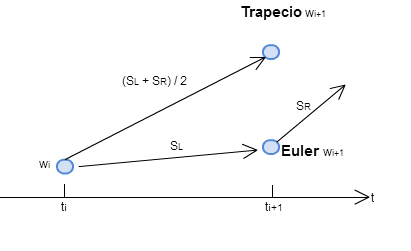
\includegraphics[width=10cm]{./Images/trapecio-vs-euler.png}
			\caption{Esquema visual del método del trapecio explícito.} 
			\label{fig:trapecio-vs-euler}
		\end{figure}

	\subsection{Método del trapecio implícito}


		Aktison

%-----------------------------------------------------------------------------------------------------
%	SECCIÓN X: ERROR
%-----------------------------------------------------------------------------------------------------


\section{Estudio del error. Convergencia}

	\subsection{Método del trapecio explícito}
	
	\subsection{Método del trapecio implícito}


%-----------------------------------------------------------------------------------------------------
%	SECCIÓN X: ESTABILIDAD
%-----------------------------------------------------------------------------------------------------

\section{Estabilidad}

%-----------------------------------------------------------------------------------------------------
%	SECCIÓN X: CONCLUSIÓN
%-----------------------------------------------------------------------------------------------------

\section{Conclusión}


%-----------------------------------------------------------------------------------------------------
%	SECCIÓN X: REFERENCIAS
%-----------------------------------------------------------------------------------------------------

\printbibliography


\end{document}